\documentclass[12pt, twoside]{article}
\usepackage[utf8]{inputenc}
\usepackage[english,russian]{babel}
\newcommand{\hdir}{.}

\usepackage{graphicx}
\usepackage{caption}
\usepackage{amssymb}
\usepackage{amsmath}
\usepackage{mathrsfs}
\usepackage{euscript}
\usepackage{upgreek}
\usepackage{array}
\usepackage{theorem}
\usepackage{graphicx}
\usepackage{subfig}
\usepackage{caption}
\usepackage{color}
\usepackage{url}

\usepackage{verbatim}

\usepackage[left=2cm,right=2cm,top=3cm,bottom=2cm,bindingoffset=0cm]{geometry}

\usepackage{fancyhdr}
\pagestyle{fancy}
\fancyhead{}
\fancyhead[LE,RO]{\thepage} 
\fancyhead[CO,CE]{Контрольная работа 2}
\fancyhead[LO,LE]{ФИО }

\begin{document} 
\section{Задача~\cite{first}}
Игровое поле $N\times M$ заполняется целыми числами, одно неотрицательное целое число в каждой клетке. Цель игры состоит в том, чтобы пройти по любому разрешенному пути от верхнего левого угла до правого нижнего. Целое число в каждой клетке указывает, какой длины шаг должен быть из текущей клетки. Все шаги могут быть или направо или вниз. Если в результати какого-либо шага игрок покидает пределы поля, такой шаг запрещается.

\begin{figure}[h!t]\center
\subfloat[]{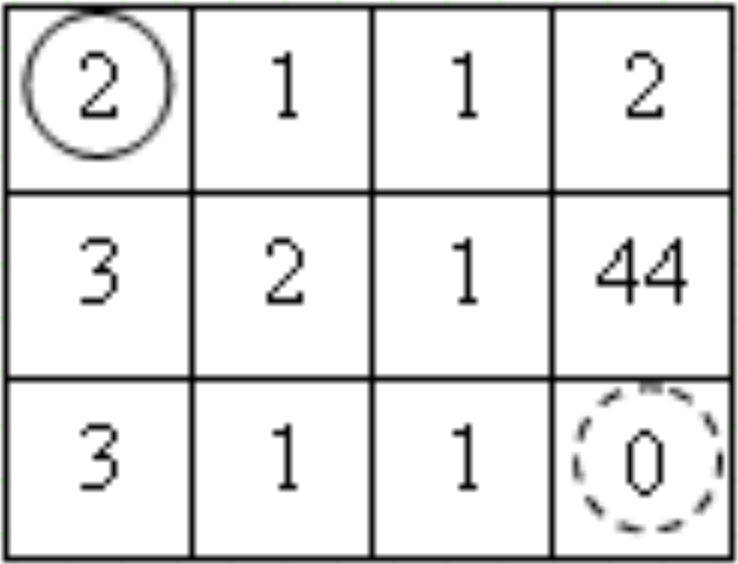
\includegraphics[width=0.2\textwidth]{1}}
\qquad~
\subfloat[]{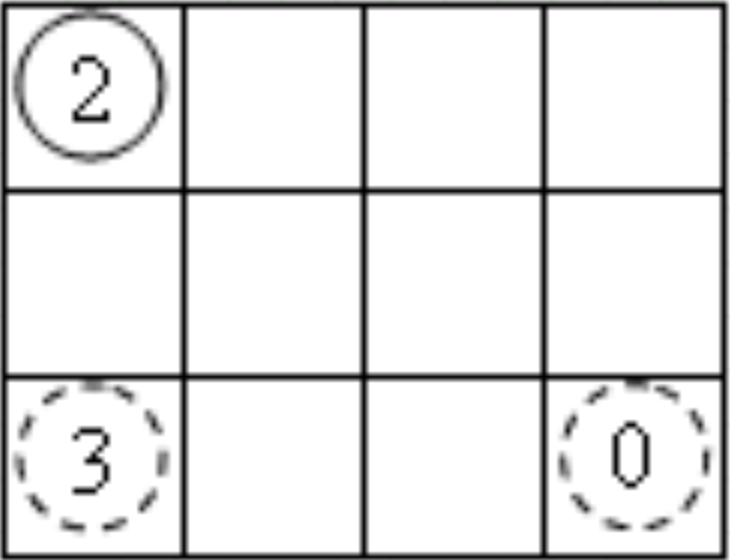
\includegraphics[width=0.2\textwidth]{2}}
\qquad~
\subfloat[]{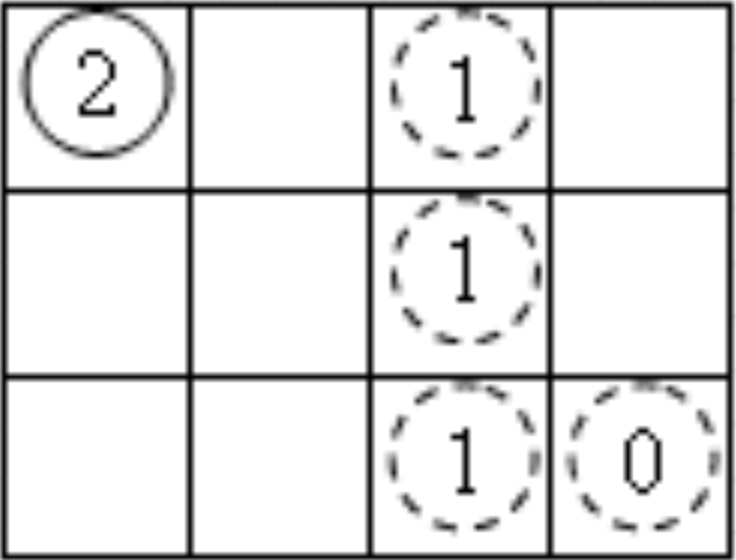
\includegraphics[width=0.2\textwidth]{3}}
\qquad~
\subfloat[]{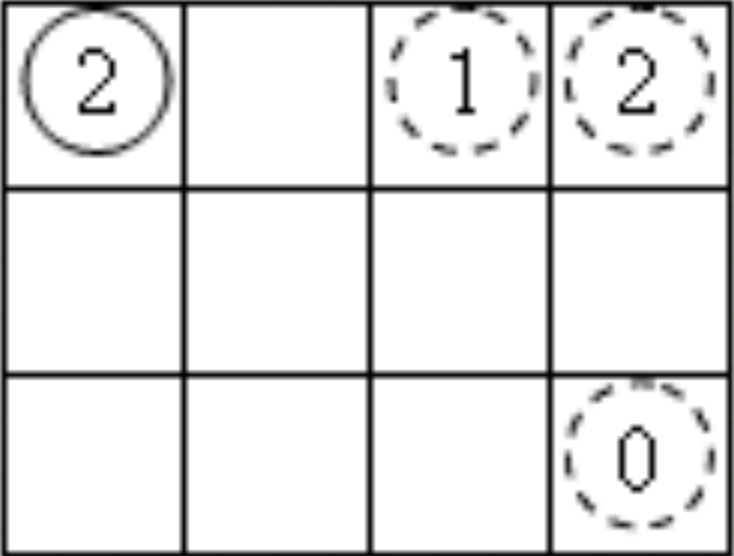
\includegraphics[width=0.2\textwidth]{4}}
\caption{пример к задаче 1}
\label{task1}
\end{figure}
На рис.~\ref{task1} приведен пример игрового поля $3\times4$, где сплошная окружность показывает положение начала, а пунктирная окружность - цели. Показывается три возможных пути от начала до цели для рассматриваемого примера игрового поля, с удаленными промежуточными числами.

Требуется написать программу, которая определит число различных вариантов путей от верхнего левого угла до правого нижнего.
\paragraph{Входные данные} содержат в первой строке размеры поля $1\leq N\leq 70~\&~1\leq M\leq 70$. В последующих $N$ строках входного файла, каждая из которых описывает отдельную строку игрового поля, записаны через пробел по $M$ целых чисел от 0 до 100 --- длины шагов из клеток данной строки.
\paragraph{Выходные данные} должны содержать одно число --- число различных вариантов путей от верзнего левого угла  до правого нижнего. Для каждого поля буде менее чем $2^{31}$ различных путей.

\begin{table}[h]
\begin{center}
\caption{Пример}
\begin{tabular}{|c|c|c|}
\hline
	 № &Входные данные& Выходные данные\\
	\hline
	
	1
	&
	\multicolumn{1}{|l|}{3 4}
	&
	3\\
	~
	&
	\multicolumn{1}{|l|}{2 1 1 2}
	&
	~\\
	~
	&
	\multicolumn{1}{|l|}{3 2 1 44}
	&
	~\\
	~
	&
	\multicolumn{1}{|l|}{3 1 1 0}
	&
	~\\
	\hline

\end{tabular}
\end{center}
\end{table}

\section{Задача~\cite{second}}
Со спутника-шпиона получено изображение в некотором волновом диапазоне сверхсекретной военной базы предполагаемого противника. База расположена в Антарктиде, все постройки на ней высечены из кубов льда и имеют на фотографии квадратную форму и не имеют общих фрагментов стен ненулевой длины. Благодаря мастерству операторов оказалась, что стены разных построек параллельны границам фотографии.

Для того, чтобы составить сверхсрочный отчет для командования. необходимо узнать, сколько зданий находятся на базе. Напишите программу, которая это сделает.
\paragraph{Входные данные} содержат в первой строке размеры фотографиии $1\leq N\leq 500~\&~1\leq M\leq 500$ в пикселях. Следующие $N$ строк содержат по $M$ символов каждая: символ '.' соответствует пустому месту, '\#' -- элементу постройки.
\paragraph{Выходные данные} содержит одно число --- число построек на базе.

\begin{table}[h]
\begin{center}
\caption{Пример}
\begin{tabular}{|c|c|c|}
\hline
	 № &Входные данные& Выходные данные\\
	\hline
	
	1
	&
	\multicolumn{1}{|l|}{8 6}
	&
	2\\
	~
	&
	\multicolumn{1}{|l|}{......}
	&
	~\\
	~
	&
	\multicolumn{1}{|l|}{...\#\#.}
	&
	~\\
	~
	&
	\multicolumn{1}{|l|}{...\#\#.}
	&
	~\\
	~
	&
	\multicolumn{1}{|l|}{......}
	&
	~\\
	~
	&
	\multicolumn{1}{|l|}{.\#\#\#..}
	&
	~\\
	~
	&
	\multicolumn{1}{|l|}{.\#\#\#..}
	&
	~\\
	~
	&
	\multicolumn{1}{|l|}{.\#\#\#..}
	&
	~\\
	~
	&
	\multicolumn{1}{|l|}{......}
	&
	~\\
	\hline

\end{tabular}
\end{center}
\end{table}



\begin{thebibliography}{99}
	\bibitem{first}
	\textit{Только вправо или вниз} {http://acmp.ru/index.asp?main=task\&id\_task=165}
	\bibitem{second}
	\textit{Военная база} {http://acmp.ru/index.asp?main=task\&id\_task=413}
\end{thebibliography}



\end{document} 



